\documentclass[convert={density=150x150},border={10pt 10pt 10pt 10pt}]{standalone}
\usepackage{amsmath, amssymb, amsthm}
\usepackage{tikz}
\usetikzlibrary{arrows,shapes,snakes,automata,backgrounds,petri}
\tikzset{n/.style={inner sep=0, minimum size=6pt, fill=black, circle}}
\begin{document}
\pagecolor{white}
  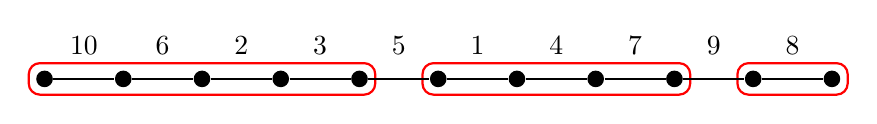
\begin{tikzpicture}
    \draw[rounded corners,draw=red,thick] (-0.2, -0.2) rectangle (4.2, 0.2);
    \draw[rounded corners,draw=red,thick] (4.8, -0.2) rectangle (8.2, 0.2);
    \draw[rounded corners,draw=red,thick] (8.8, -0.2) rectangle (10.2, 0.2);

    \foreach \x in {0,1,...,10}
    {
      \node[n](A\x) at (\x, 0) {};
    }
    \def\testarray{{10,6,2,3,5,1,4,7,9,8}}
    \foreach \x in {0,1,...,9}
    {
      \pgfmathparse{int(\x+1)}
      \edef\y{\pgfmathresult}%
      \pgfmathparse{\testarray[\x]}
      \edef\v{\pgfmathresult}
      \draw[thick] (A\x) -- (A\y) node [midway, above, yshift=5pt] {$\v$};
    }
    

  \end{tikzpicture}
\end{document}